\subsection{19. Нормальная форма Грейбах для КС-грамматик. Модифицированный алгоритм Кока-Янгера-Касами для нормальной формы Грейбах: достоинства и недостатки.}

\Def Грамматика в нормальной форме Грейбах (grammar in Greibach normal form) — контекстно-свободная грамматика $\langle N, \Sigma, P, S \rangle$, в которой каждое правило имеет один из следующих четырёх видов:

1) $S \rightarrow \varepsilon$

2) $A \rightarrow a$

3) $A \rightarrow aB$

4) $A \rightarrow aBC$

причём $B, C \in N$, $B, C \neq S$, $a \in \Sigma$\\

\textbf{Модифицированный алгоритм Кока-Янгера-Касами}

Утверждение: проще парсить из нормальной формы Грейбаха, т.к. каждый раз мы вытаскиваем одну букву $\Rightarrow$ в алгоритме Кока-Янгера-Касами константа будет ниже; 

Минус: большое количество нетерминалов.\\


\textbf{Теорема} Каждая контекстно-свободная грамматика
эквивалентна некоторой грамматике в нормальной форме
Грейбах. (на хор 6 и выше по версии Виталия)

$\blacktriangle$
0. Возьмём G в НФ Хомского. Введём обозначение: $A \backslash B \vdash w \Leftrightarrow A \vdash Bw$

1. Заметим следующее:

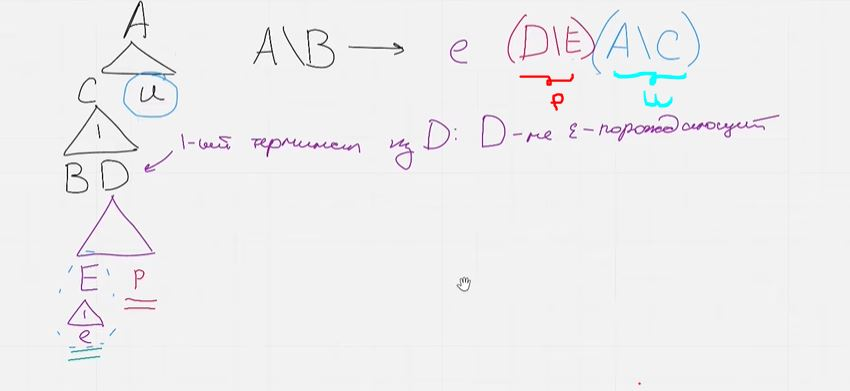
\includegraphics[width=15cm]{images/greybach.JPG}

2. Вводим G' =  $\langle N', \Sigma, P', S \rangle$, где $N' = \{S\} \cup \{(A \backslash B) | A, B \in N\}$, 

а $P' = \{(A \backslash A) \rightarrow \varepsilon | A \in N \} \cup \{ S \rightarrow a(S \backslash A) | A \rightarrow a \in P\} \cup \{ (A \backslash B) \rightarrow e (D \backslash E) (A \backslash C) | C \rightarrow BD, E \rightarrow e \in P\} \cup \{ S \rightarrow \varepsilon | S \rightarrow \varepsilon \in P\}$. Отсюда $O(N') = O(N^2)$
$\blacksquare$

Осталось доказать: $\forall A, B \in N$ $\forall w \in \Sigma^*$   $A \vdash_G Bw \Leftrightarrow (A \backslash B) \vdash_{G'} w$

$\Rightarrow$: индукция по длине вывода в G. База: A = B, $w = \varepsilon$. Переход: см. картинку

$\Leftarrow$: индукция по длине вывода в G'. База: $A\backslash B \vdash_1 w \Rightarrow w = \varepsilon, A = B \Rightarrow A \vdash A \varepsilon$.

Переход:  $A\backslash B \vdash_1 e(C \backslash D)(A \backslash F)$; $(C \backslash D) \vdash u$; по предположению индукции, $C \vdash Du$. Аналогично, $A \vdash Fv$. + в P есть правила $D \rightarrow e$ и $F \rightarrow BC$.

Тогда $A \vdash Fv \vdash BCv \vdash BDuv \vdash Beuv$. Почти победа!

\textbf{L(G) = L(G')}. $w \in L(G) \Leftrightarrow S \vdash w$.

$L(G) \subset L(G')$: пусть $S \vdash w$

1) $w = \varepsilon$, переносим правило $S \rightarrow \varepsilon$ в G'

2) $w \neq \varepsilon$. Тогда $w = au$. $S \vdash Au \vdash_1 au$, т.к. НФ Хомского. По лемме $S \backslash A \vdash u$ $\Longrightarrow S \vdash_{G'} a(S \backslash A) \vdash au = w$. 

$L(G') \subset L(G)$:  $w= au$, $S \vdash_{G'} a(S \backslash A)$, где $ A \rightarrow a \in P$, тогда $S \backslash A \vdash u$, в итоге $S \vdash Au = au = w$.
